Da der Naschmarkt in dem Framework Laravel geschrieben ist, folgt es dem MVC Prinzip.

\begin{figure}[H]
	\begin{center}
		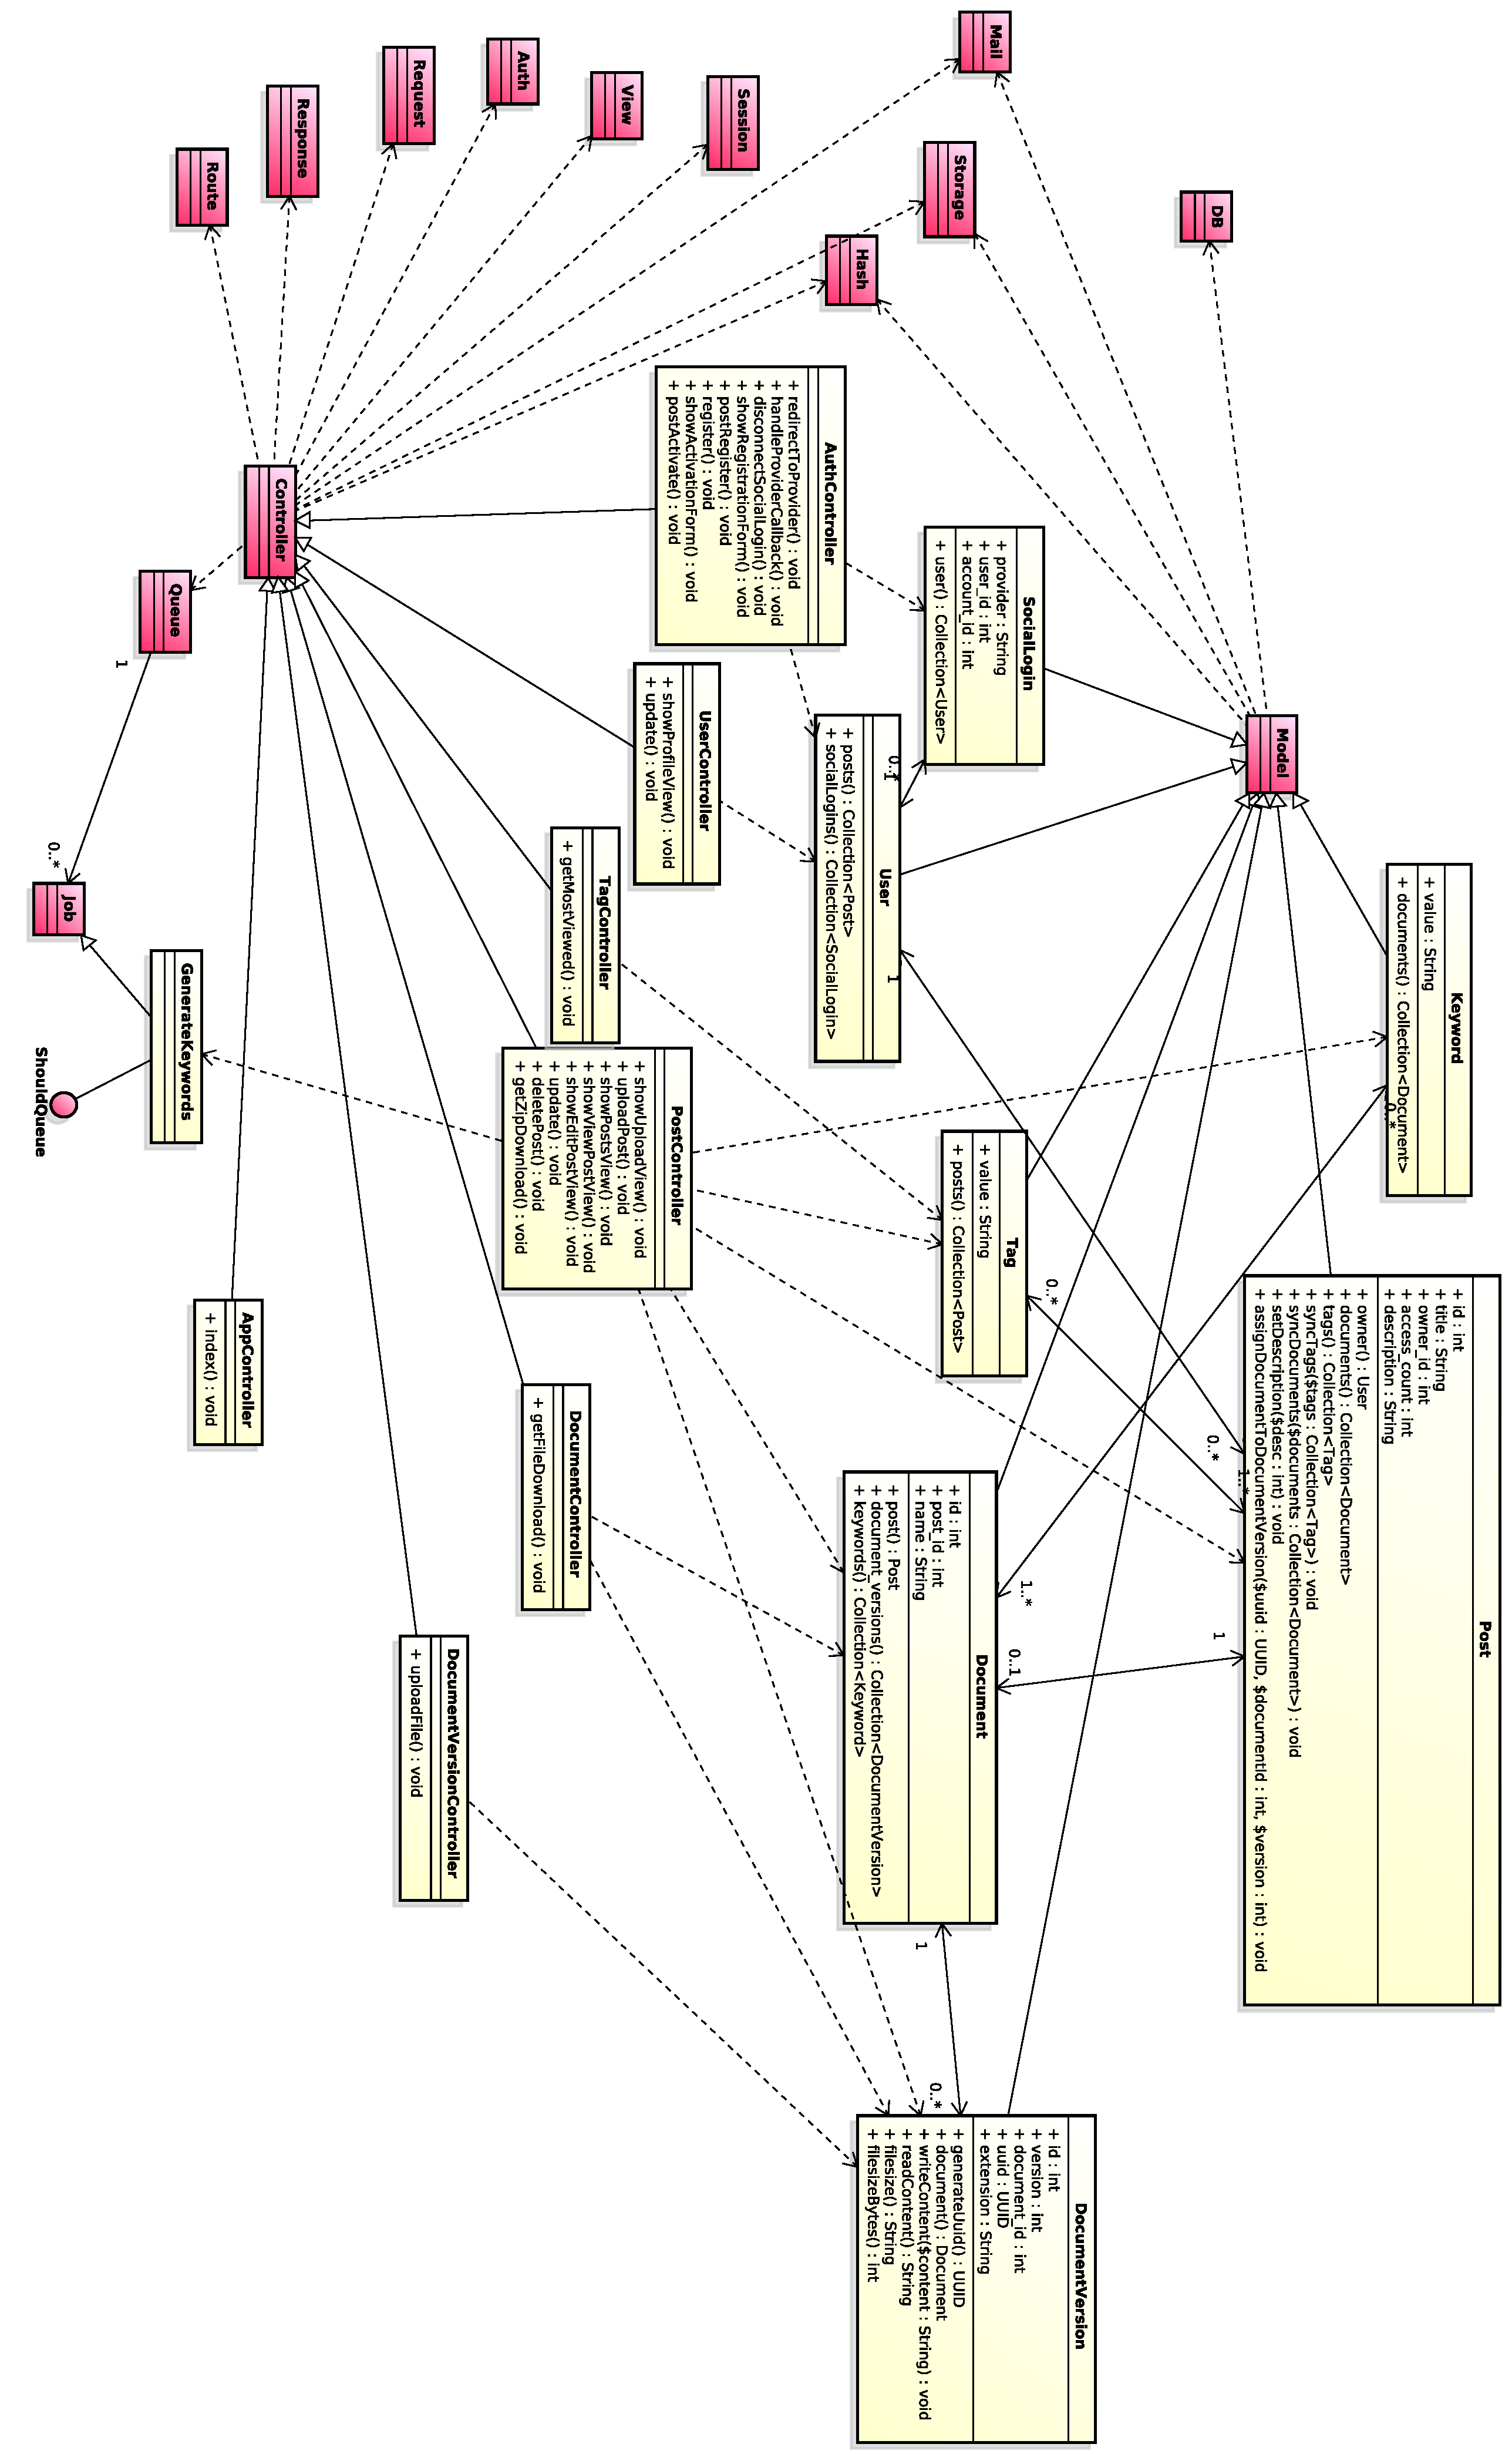
\includegraphics[width=\linewidth]{images/UML_Classdiagramm.pdf}
		\caption{UML Diagramm}
	\end{center}
\end{figure}

In der folgenden Graphik sind die M\"oglichkeiten des Projektes beschrieben in einem Use-Case Diagramm.

\begin{figure}[H]
	\begin{center}
		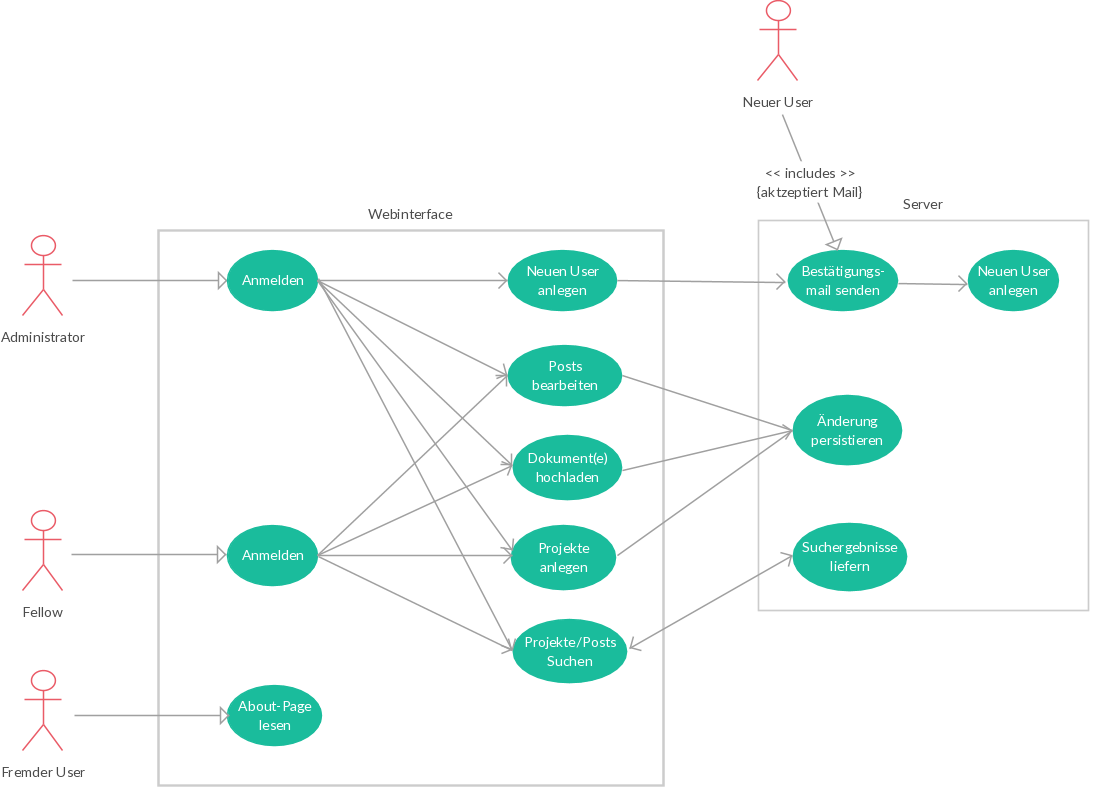
\includegraphics[width=\linewidth]{images/use_case.png}
		\caption{Use Case Diagramm}
	\end{center}
\end{figure}
